\documentclass{beamer}
\beamertemplatenavigationsymbolsempty
\usecolortheme{beaver}
\setbeamertemplate{blocks}[rounded=true, shadow=true]
\setbeamertemplate{footline}[page number]
%
\usepackage[utf8]{inputenc}
\usepackage[english,russian]{babel}
\usepackage{amssymb,amsfonts,amsmath,mathtext}
\usepackage{subfig}
\usepackage[all]{xy} % xy package for diagrams
\usepackage{array}
\usepackage{multicol}% many columns in slide
\usepackage{hyperref}% urls
\usepackage{hhline}%tables
\usepackage{algorithm}
\usepackage{algpseudocode}
\usepackage{xspace}
% Your figures are here:
\graphicspath{ {fig/} {../figures/} }

%----------------------------------------------------------------------------------------------------------
\title[\hbox to 56mm{Малоранговые разложения в распределенном обучении}]{Методы малоранговых разложений в распределенном и федеративном обучении}
\author[А.\,В. Ребриков]{Алексей Витальевич Ребриков}
\institute{Московский физико-технический институт}
\date{\footnotesize
\par\smallskip\emph{Курс:} Автоматизация научных исследований\par (практика, В.\,В.~Стрижов)/Группа 105
\par\smallskip\emph{Эксперт:} к.ф.-м.н. А.\,Н.~Безносиков
\par\smallskip\emph{Консультант:} А.\,В.~Зыль
\par\bigskip\small 2024}
%----------------------------------------------------------------------------------------------------------
\begin{document}
%----------------------------------------------------------------------------------------------------------
\begin{frame}
\thispagestyle{empty}
\maketitle
\end{frame}
\newcommand{\R}{\mathbb{R}}
\newcommand{\cC}{\mathcal{C}}
\def\stepsize{\eta}
%-----------------------------------------------------------------------------------------------------
\begin{frame}{Цель исследования}
\begin{block}{Решается задача}
    распределённой оптимизации с использованием EF21
    \begin{align*}
        \min \limits_{x \in \R^d} \left\{ f(x) = \frac{1}{n} \sum \limits_{i=1}^n f_i(x) \right\}
        \qquad
        x^{k+1} = x^k - \frac{\stepsize^k}{n} \sum \limits_{i=1}^n \nabla f_i(x^k)
    \end{align*} 
\end{block}
\begin{block}{Основная идея}
    сжатие градиентов с использованием малоранговых разложений (например HOSVD)
\end{block}
\begin{block}{Цель}
    сравнить известные операторы сжатия с новыми
\end{block}
\end{frame}
%-----------------------------------------------------------------------------------------------------

\begin{frame}{Доклад с одним слайдом}
\begin{columns}[c]
\column{0.4\textwidth}
\begin{align*}
    \min \limits_{x \in \R^d} \left\{ f(x) = \frac{1}{n} \sum \limits_{i=1}^n f_i(x) \right\}
    \end{align*}

    \textbf{Ключевые пункты:}
    \begin{enumerate}
        \item Данные распределяются.
        \item Веса модели общие.
        \item Передача градиентов сжимается.
        \item Сжимается не сам градиент, а его разность. (EF21)
    \end{enumerate}

\column{0.6\textwidth}
\begin{figure}
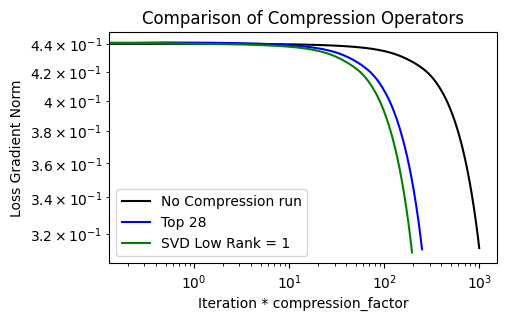
\includegraphics[width=1.0\textwidth]{output1.png}
\end{figure}\begin{figure}
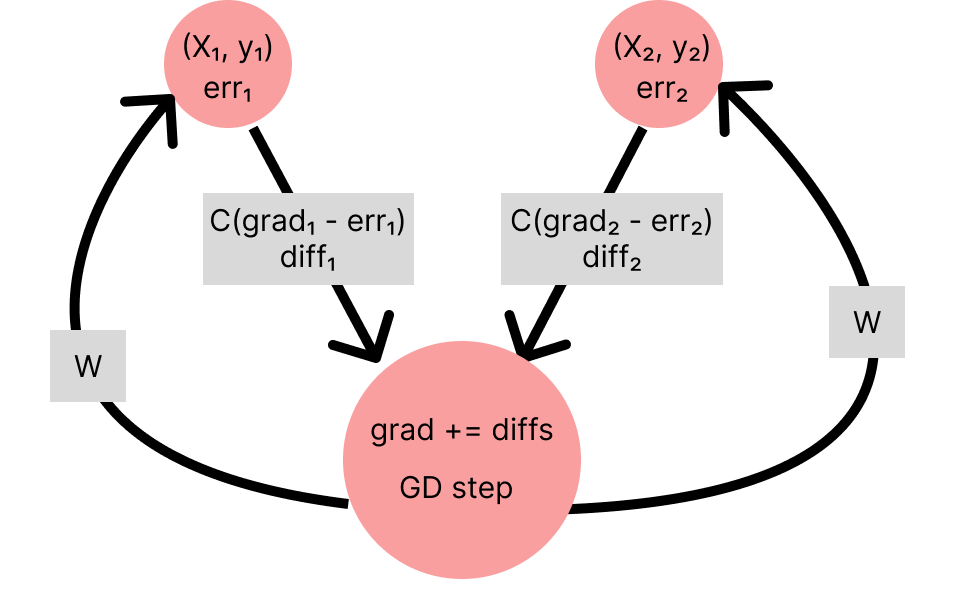
\includegraphics[width=0.8\textwidth]{img3.png}
\end{figure}

\end{columns}

\end{frame}
\newcommand{\sqnorm}[1]{\left\lVert#1\right\rVert^2}
\newcommand{\algname}[1]{{\sf \footnotesize #1}\xspace}


%----------------------------------------------------------------------------------------------------------
\begin{frame}{Литература}
    \small
    \bibliographystyle{apalike}
    \nocite{richtarik2021ef21,de2000multilinear,beznosikov2023biased}
    \bibliography{../paper/Rebrikov2024LowRankDistFedLearning}
\end{frame}
%----------------------------------------------------------------------------------------------------------
\begin{frame}{EF21}
    \begin{algorithm}[H]
        \small
        \centering
        \caption{\algname{EF21} (Multiple nodes)}\label{alg:EF21}
        \begin{algorithmic}[1]
            \State \textbf{Input:} starting point $x^{0} \in \R^d$;  $g_i^0 = \cC(\nabla f_i(x^0))$ for $i=1,\dots, n$ (known by nodes and the master); learning rate $\gamma>0$; $g^0 = \frac{1}{n}\sum_{i=1}^n g_i^0$ (known by master)
            \For{$t=0,1, 2, \dots , T-1 $}
            \State Master computes $x^{t+1} = x^t - \gamma g^t$ and broadcasts $x^{t+1}$ to all nodes
            \For{{\bf all nodes $i =1,\dots, n$ in parallel}}
            \State Compress $c_i^t = \cC(\nabla f_i(x^{t+1}) - g_i^t)$ and send $c_i^t $ to the master
            \State Update local state $g_i^{t+1} = g_i^t + \cC( \nabla f_i(x^{t+1}) - g_i^t)$
            \EndFor
            \State Master computes $g^{t+1} = \frac{1}{n} \sum_{i=1}^n  g_i^{t+1}$ via  $g^{t+1} = g^t + \frac{1}{n} \sum_{i=1}^n c_i^t $
            \EndFor
        \end{algorithmic}
    \end{algorithm}
    \cite{richtarik2021ef21}
\end{frame}

% \newcommand{\R}{\mathbb{R}}
% \newcommand{\cC}{\mathcal{C}}
\newcommand{\T}{\mathcal{T}}
\begin{frame}{Оператор сжатия HOSVD}

    \small
    \begin{block}{Определение}
        Под оператором сжатия понимается (возможно стохастическое) отображение $\cC : \R^d \rightarrow \R^d$, которое удовлетворяет определённым ограничениям на изменение информации.
    \end{block}

    \begin{algorithm}[H]
        \small
        \centering
        \caption{Алгоритм сжатия данных с использованием HOSVD}
        \begin{algorithmic}[1]
            \State \textbf{Input:} vector $x \in \R^d$.
            \State Reshape the vector $x$ into a tensor $\T(x) = \text{reshape}(x, \text{dims})$.
            \State Apply HOSVD to the tensor $\T(x)$ to obtain its decomposition.
            \State Truncate the ranks of the tensor decomposition to $(r_1, r_2, \dots, r_k)$.
            \State Send the compressed tensor to the master.
            \State Master reconstructs the full tensor from its decomposition.
            \State Master reshapes the tensor back into the vector form.
        \end{algorithmic}        
    \end{algorithm}
\end{frame}
%----------------------------------------------------------------------------------------------------------
% \begin{frame}{Решение}
% \begin{columns}[c]
% \column{0.6\textwidth}
%     Столбец 1
% \column{0.4\textwidth}
%     Столбец 2
% \end{columns}
% \end{frame}
%----------------------------------------------------------------------------------------------------------
\begin{frame}{Вычислительный эксперимент}
\small
 Сравнение нормы градиента от величины пропорциональной переданной информации
\begin{figure}
    \centering
    
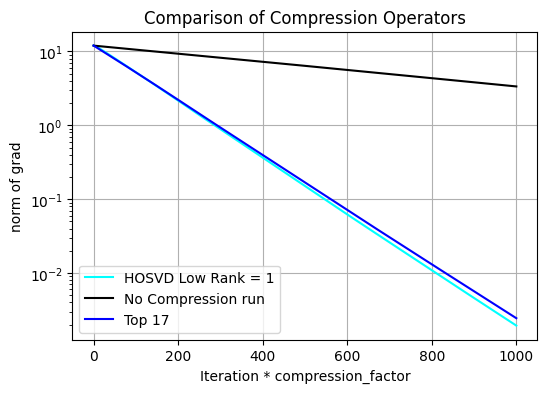
\includegraphics[width=0.8\textwidth]{../figures/hosvd.png}
\end{figure}

HOSVD оператор работает наравне с используемым top-k

\end{frame}
%----------------------------------------------------------------------------------------------------------
\begin{frame}{Заключение}
    \begin{block}{Результаты}
    \begin{itemize}
        \item предложен новый метод сжатия,
        \item проведено сравнение с Top-k \cite{alistarh2018convergence}
    \end{itemize}
    \end{block}
    \begin{block}{Будущаяя работа}
    \begin{itemize}
        \item перенести код на PyTorch,
        \item применить для сложных сетей (свёрточных),
        \item исследовать другие разложения (TT, Tucker, etc.)
    \end{itemize}
    \end{block}
\end{frame}
%----------------------------------------------------------------------------------------------------------




\end{document} 